\begin{figure}[ht]
	\begin{center}
	\tikzsetnextfilename{plot_aufteilung_integral}
		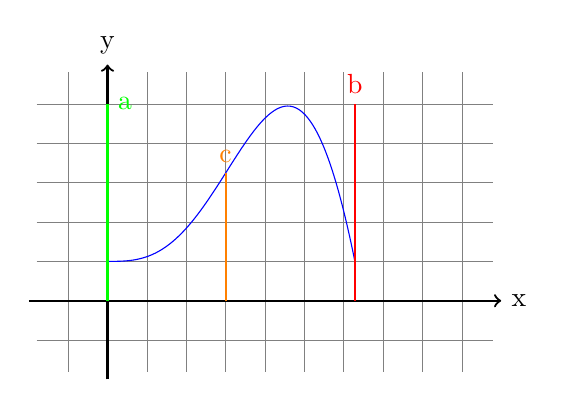
\begin{tikzpicture}
			\draw[very thin, gray, step = 0.5] (-0.9,-0.9) grid (4.9,2.9);
			\draw[->,thick, black](-1,0) -- (5,0) node[right]{x};
			\draw[->,thick, black](0,-1) -- (0,3) node[above]{y};
			\draw[blue,domain = 0.0:3.14, samples=1000]   
				plot (\x,{(\x * \x)*sin(\x r)*0.5+0.5});
	       	\draw[green,thick](0.0,0)--(0.0,2.5)node[right]{a};
	       	\draw[red,thick](3.14,0) -- (3.14,2.5) node[above]{b};
	       	\draw[orange,thick](1.5,0) -- (1.5, 1.62) node[above]{c};
		\end{tikzpicture}
	\end{center}
	\caption{Integral aufteilen}
	\label{fig_integral_aufteilen}
\end{figure}